\chapter{Programiranje sistema}

\section{Arduino kôd}
Arduino programski jezik temelji se na Wiring programskom okviru za upravljanje mikrokontrolerima, a Arduino softver temelji se na Processing softveru. Wiring je sličan C++ programskom jeziku, ali je djelomično pojednostavljen i izmijenjen. Wiring i Processing su, kao i Arduino, \textit{open source}, odnosno otvorenog kôda, dostupni besplatno, zajedno sa svim projektima i doprinosima korisnika.

Cijeli programski kôd ovog sistema dan je prilogu. On se sastoji od uvođenja svih biblioteka potrebnih za rad, deklarisanja varijabli, funkcija za rad pojedinih dijelova, te \textit{setup()} i \textit{loop()} funkcija. U \textit{setup()} funkciji su sve radnje koje se pokreću čim se mikrokontroler pokrene, a u \textit{loop()} funkciji radnje koje se ponavljaju beskonačno mnogo puta dok god mikrokontroler ima ulazni napon.  

Ono što se u ovom sistemu beskonačno mnogo puta ponavlja je čitanje podataka koji se primaju preko Bluetootha. 
Loop se neprestano vrti dok god je pločica priključena na napon. Tu se čitaju primljeni podaci s bluetooth senzora, i prema njima pokreću funkcije. Ako je korisnik pritisnuo button za pokretanje vrteške, ona se počne vrtiti, ako je pritisnuo za zaustavljanje, ona stane, i tako dalje.
 \begin{lstlisting}[frame=single,language=C++,numbers=left, numberstyle=\tiny, xleftmargin=0.05\textwidth, xrightmargin=0.05\textwidth, basicstyle=\ttfamily\footnotesize]
 void loop(){
 
while(Serial1.available()==0) ;

if(Serial1.available()>0) {
data = Serial1.parseInt();
 
} 

delay(400);

\end{lstlisting}

U varijablu \textit{data} spremaju se brojevi primljeni preko bluetooth senzora. Njihova vrijednost je definisana u aplikaciji napravljenoj pomoću Android studija. U toj aplikaciji, na primjer, ako korisnik pritisne button za uključenje dioda, preko Bluetootha se šalje broj 67, a ako pritisne button za gašenje dioda, preko bluetootha se šalje broj 76. Shodno tome, aplikacija mikrokontrolera, ako primi broj 67, treba uključiti diode, a ako primi broj 76, treba ih isključiti.
 \begin{lstlisting}[frame=single,language=C++,numbers=left, numberstyle=\tiny, xleftmargin=0.05\textwidth, xrightmargin=0.05\textwidth, basicstyle=\ttfamily\footnotesize]
 if (data == 67){
  diodeUkljuci();
}
if (data == 76){
  diodeIskljuci();
}

\end{lstlisting}

Na analogan način je napravljena veza između aplikacije i svih drugih dijelova sistema, samo, naravno, sa različitim vrijednostima koje se šalju preko bluetootha.
 \begin{lstlisting}[frame=single,language=C++,numbers=left, numberstyle=\tiny, xleftmargin=0.05\textwidth, xrightmargin=0.05\textwidth, basicstyle=\ttfamily\footnotesize]
if (data == 23){
  vracara();
}
if (data == 32){
  vracaraUgasi();
}
\end{lstlisting}

Vračara ima svoju kristalnu kuglu, čije se boje mijenjaju promjenom boja RGB diode.
   \begin{lstlisting}[frame=single,language=C++,numbers=left, numberstyle=\tiny, xleftmargin=0.05\textwidth, xrightmargin=0.05\textwidth, basicstyle=\ttfamily\footnotesize] 
void vracara(){
  RGB_color(255, 0, 0); // crvena
  delay(1000);
  RGB_color(0, 255, 0); // zelena
  delay(1000);
  RGB_color(0, 0, 255); // plava
  delay(1000);
  RGB_color(255, 255, 125); // roza
  delay(1000);
  RGB_color(0, 255, 255); // cijan
  delay(1000);
  RGB_color(255, 0, 255); // magenta
  delay(1000);
  RGB_color(255, 255, 0); // zuta
  delay(1000);
  RGB_color(255, 255, 255); // bijela
  delay(1000);
}


void RGB_color(int crvena, int zelena, int plava) {
  analogWrite(crveni_pin, crvena);
  analogWrite(zeleni_pin, zelena);
  analogWrite(plavi_pin, plava);
}
 \end{lstlisting}
 
Senzor za boje osvijetli lopticu uz pomoć jedne od tri diode, prvo crvene (R), pa zelene (G), pa plave (B), a onda čita vrijednost dobijene frekvencije da dobije zastupljenost boje koju ta dioda emitira na loptici.

 \begin{lstlisting}[frame=single,language=C++,numbers=left, numberstyle=\tiny, xleftmargin=0.05\textwidth, xrightmargin=0.05\textwidth, basicstyle=\ttfamily\footnotesize]
int readColor() {
// Citanje crvenih fotodioda
  digitalWrite(S2, LOW);
  digitalWrite(S3, LOW);
  frekvencija = pulseIn(sensorOut, LOW);
  int R = frekvencija;
    delay(50);

// Citanje zelenih fotodioda
  digitalWrite(S2, HIGH);
  digitalWrite(S3, HIGH);
  frekvencija = pulseIn(sensorOut, LOW);
  int G = frekvencija;
  delay(50);
  
// Citanje plavih fotodioda
  digitalWrite(S2, LOW);
  digitalWrite(S3, HIGH);
  frekvencija = pulseIn(sensorOut, LOW);
  int B = frekvencja;
  delay(50);

  if((R<45 & R>32 & G<70 & G>50) || (R>70 & G<10 & B <50 & B>30) ){
    color = 1; // Crvena
  }
  if(R<45 & R>35 & B<40 &B>30){
    color = 2; // Roza
  }
  if(R<63 & R>50 & G<55 & G>45 & B<40 & B>29){
    color = 3; // Plava
  }
  if(R<40 & R>30 & G<50 & G>40 & B<46 & B>38){
    color = 4; // Zuta
  }
  return color;  
}
 \end{lstlisting}

Ako je pritisnut jedan od buttona, pokrese se dio programa. Ako korisnik pritisne odgovarajući button, te pogodi koje je boje loptica, on pobijedi, uključuje se zelena dioda, u suprotnom, uključuje se crvena. Loptica se uz pomoć servo motora i napravljenog mehanizma kreće, prvo do senzora za boju, gdje se očita njena boja, a onda u odgovarajuću posudu.

 \begin{lstlisting}[frame=single,language=C++,numbers=left, numberstyle=\tiny, xleftmargin=0.05\textwidth, xrightmargin=0.05\textwidth, basicstyle=\ttfamily\footnotesize]
void senzorZaBoje(){
   crveniButtonState = digitalRead(crveniButton);
   plaviButtonState = digitalRead(plaviButton);


  if (crveniButtonState == HIGH || plaviButtonState == HIGH) {
  gornjiServo.write(120);
  delay(3000);
  
  for(int i = 115; i > 55; i--) {
    gornjiServo.write(i);
    delay(2);
  }
  delay(1000);
  
  color = readColor();
  color = readColor();
  color = readColor();
  color = readColor();
  
  delay(1000);  
  switch (color) {
    case 1: //crvena
    if (crveniButtonState == HIGH){
      digitalWrite(zelenaDioda, HIGH);
      digitalWrite(crvenaDioda, LOW);
    }
    if (plaviButtonState == HIGH ){
      digitalWrite(crvenaDioda, HIGH);
      digitalWrite(zelenaDioda, LOW);
    }
    donjiServo.write(50);
    break;
    case 2: //roza
    digitalWrite(crvenaDioda, HIGH);
    digitalWrite(zelenaDioda, LOW);
    donjiServo.write(75);
    break;
    case 3: // zuta
      digitalWrite(crvenaDioda, HIGH);
      digitalWrite(zelenaDioda, LOW);
    donjiServo.write(100);
    break;
    case 4: // plava
     if (plaviButtonState == HIGH){
    digitalWrite(zelenaDioda, HIGH);
    digitalWrite(crvenaDioda, LOW);
    }
    if (crveniButtonState == HIGH ){
    digitalWrite(crvenaDioda, HIGH);
    digitalWrite(zelenaDioda, LOW);
    }
    donjiServo.write(125);
    break;  
    case 0:
    break;
  }
  delay(300);
  
  for(int i = 55; i > 20; i--) {
    gornjiServo.write(i);
    delay(2);
  } 
  delay(500);
  
  for(int i = 29; i < 115; i++) {
    gornjiServo.write(i);
    delay(2);
  }
  color=0;
  }
}
 \end{lstlisting}
 Motori se vrte stavljanjem pozitivnih i negativnih napona na njihove pinove.

 \begin{lstlisting}[frame=single,language=C++,numbers=left, numberstyle=\tiny, xleftmargin=0.05\textwidth, xrightmargin=0.05\textwidth, basicstyle=\ttfamily\footnotesize]
void vrtiMotore(){
  digitalWrite(motor1pin1, HIGH);
  digitalWrite(motor1pin2, LOW);

  digitalWrite(motor2pin1, HIGH);
  digitalWrite(motor2pin2, LOW);

  digitalWrite(motor3pin1, HIGH);
  digitalWrite(motor3pin2, LOW);
  
    analogWrite(enA, 160);  // upravljanje brzinom
  digitalWrite(motor4pin1, HIGH);
  digitalWrite(motor4pin2, LOW);
}
 \end{lstlisting}
 Na ovaj način isprogramiran je svaki dio sistema.

\section{Android Studio kôd}
Sve mobilne aplikacije napravljene uz pomoć softvera Android Studio sastoje se od takozvanih aktivnosti (eng. \textit{activities}). Jedna aktivnost predstavlja jednu radnju, koja najčešće zauzima cijeli ekran. Iz jedne aktivnosti u drugu prelazi se automatski, ili aktiviranjem nekog linka ili tipke na ekranu.

Prvi dio aplikacije napravljen je uz pomoć biblioteke od Tensorflowa za treniranje neuronske mreže, te prepoznavanje treniranih objekata u Android aplikaciji. Prepoznavanje slike je akcija kojom uređaj, koji izvrši akviziciju slike, u ovom slučaju preko kamere kao ulaza, prepozna koji je objekat na istoj, te ispiše kojoj klasi pripada. Moderni načini prepoznavanja slike su korištenjem dubokog učenja, odnosno, treniranjem konvolutivnih neuronskih mreža na ogromnim bazama podataka. Tensorflow, korišten za izradu programa, je \textit{open-source} platforma, odnosno platforma otvorenog kôda, za mašinsko učenje koja sadrži ogroman broj alata i biblioteka za olakšani razvoj aplikacija. Ovu platformu je razvio Google Brain, Googleov tim za umjetnu inteligenciju, prvotno samo za potrebe kompanije Google, a u novembru 2015. godine objavljen je za široku populaciju pod Apache 2.0 licencom. Može se koristiti za kreiranje algoritama za mašinsko učenje, te za pokretanje istih, a bez puno promjena može se pokrenuti na mnogim uređajima, od mobilnih telefona i tableta do velikih distribuiranih sistema sastavljenih od stotina ili hiljada uređaja poput GPU kartica \cite{Tensorflow}. 

Klasifikator za prepoznavanje slika u ovom projektu napravljen je treniranjem jednostavnog modela uz pomoć dubokog učenja sa online alatom kojeg je razvio Google, a koji se zove Teachable Machine. Treniranje modela prikazano je na slici \ref{fig:Slika_Treniranje}, a isti je eksportovan u TensorFlow lite datoteku, koja se može koristiti na Android uređajima.
\begin{figure}[h!]
  \centering
  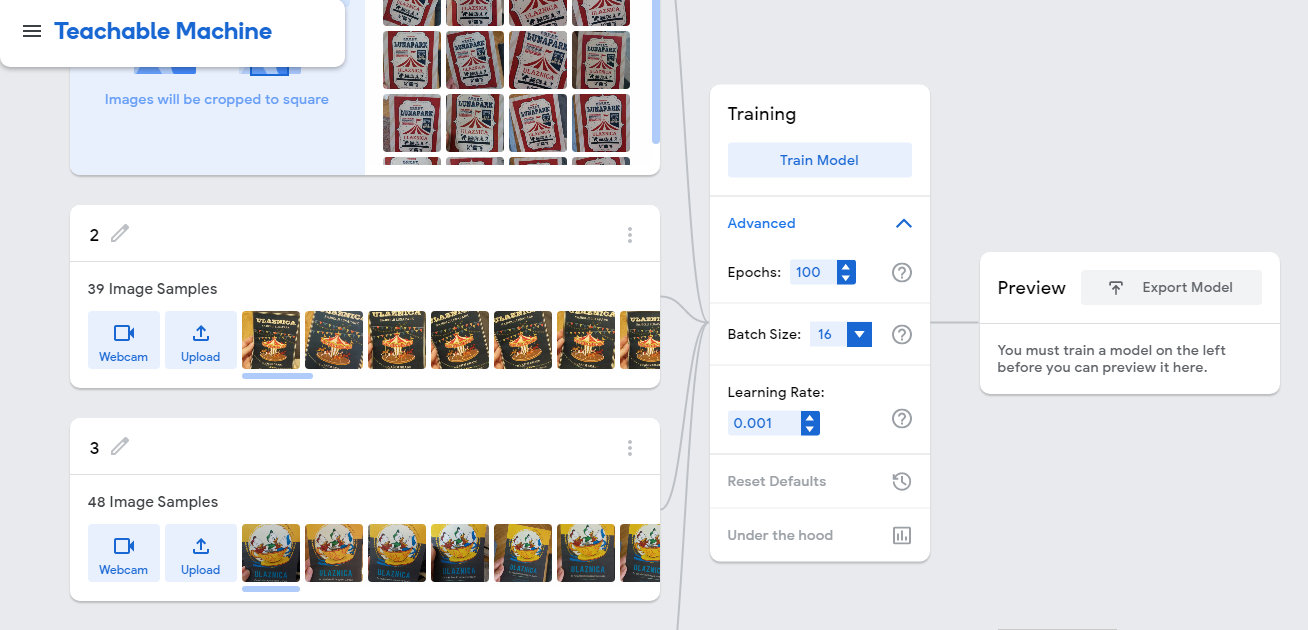
\includegraphics[width=0.8\textwidth]{treniranje.png}
  \caption{Treniranje neuronske mreže}
  \label{fig:Slika_Treniranje}
\end{figure}

Model se sastoji od slika ulaznica za lunapark, koje su kreirane u softveru Adobe Photoshop. Za projekat su napravljene 4 ulaznice, a njihove fotografije raspoređene su u 4 direktorija pomoću kojih je neuronska mreža istrenirana. TensorFlow nudi vlastitu aplikaciju otvorenog kôda za korištenje modela. Ista je izmijenjena da se prilagodi potrebama projekta.

Prvo što se korisniku prikaže je izlaz iz kamere njegovog mobitela, te poruka da pokaže ulaznicu. Bitan dio kôda je:

\begin{lstlisting}[frame=single,language=Java,numbers=left, numberstyle=\tiny, xleftmargin=0.05\textwidth, xrightmargin=0.05\textwidth, basicstyle=\ttfamily\footnotesize]
 protected void showResultsInBottomSheet(List<Recognition> results) {
    if (results != null && results.size() >= 3) {

      Recognition recognition = results.get(0);
      if (recognition != null) {

        if (recognition.getTitle() != null)
          recognitionTextView.setText(recognition.getTitle());
        System.out.println("name"+recognition.getTitle());

        System.out.println("namevalue"+recognition.getConfidence());
        if(recognition.getConfidence()<0.90f){
          result_text.setText("Pokazite ulaznicu"); 
          // ako je stepen prepoznavanja manji od 0.9, korisniku se ispisuje poruka da pokaze ulaznicu
        }
          if(recognition.getConfidence()>0.90f){
            result_text.setText(recognition.getTitle());
            Intent intent = new Intent(getApplicationContext(), BtActivity.class);
            startActivity(intent);
            // ako je stepen prepoznavanja veci od 0.9, korisnika se prebacuje na Bluetooth aktivnost
          }
          }
          \end{lstlisting}

Kad sistem prepozna ulaznicu, pokrene se sljedeća aktivnost, a to je izbornik za traženje dostupnih Bluetooth uređaja, te povezivanje na odgovarajući. Sastoji se od dva buttona, odnosno dugmeta, tipke, te liste Bluetooth uređaja koja nije vidljiva dok korisnik ne pokrene pretragu.

Kad korisnik dodirne dugme za pretragu, ispiše mu se lista dostupnih bluetooth uređaja:

\begin{lstlisting}[frame=single,language=Java,numbers=left, numberstyle=\tiny, xleftmargin=0.05\textwidth, xrightmargin=0.05\textwidth, basicstyle=\ttfamily\footnotesize]
pretraga.setOnClickListener(new View.OnClickListener() {

            @Override
            public void onClick(View arg0) {
                mBTAdapter = BluetoothAdapter.getDefaultAdapter(); // povezivanje na bluetooth adapter

                if (mBTAdapter == null) {
                    Toast.makeText(getApplicationContext(), "Bluetooth uredajii nisu pronadeni", Toast.LENGTH_SHORT).show(); // poruka ako nije pronaden ni jedan uredaj
                } else if (!mBTAdapter.isEnabled()) {
                    Intent enableBT = new Intent(BluetoothAdapter.ACTION_REQUEST_ENABLE);
                    startActivityForResult(enableBT, BT_ENABLE_REQUEST);
                } else {
                    new SearchDevices().execute(); // pretraga uredeja
                }
            }
        });
        \end{lstlisting}
 Ako korisnik nije povezan na bluetooth, otvori se poruka da ga je potrebno uključiti. Pretraga uređaja vrši se sljedećim dijelom kôda:
        \begin{lstlisting}[frame=single,language=Java,numbers=left, numberstyle=\tiny, xleftmargin=0.05\textwidth, xrightmargin=0.05\textwidth, basicstyle=\ttfamily\footnotesize]
   private class SearchDevices extends AsyncTask<Void, Void, List<BluetoothDevice>> {

        @Override
        protected List<BluetoothDevice> doInBackground(Void... params) {
            Set<BluetoothDevice> pairedDevices = mBTAdapter.getBondedDevices();
            List<BluetoothDevice> listDevices = new ArrayList<BluetoothDevice>(); // kreiranje liste
            for (BluetoothDevice device : pairedDevices) {
                listDevices.add(device); // stavljanje uredaja u listu
            }
            return listDevices;

        }
\end{lstlisting}

Kad korisnik klikne na dugme za povezivanje, pokrene se povezivanje na odabrani bluetooth uređaj:

\begin{lstlisting}[frame=single,language=Java,numbers=left, numberstyle=\tiny, xleftmargin=0.05\textwidth, xrightmargin=0.05\textwidth, basicstyle=\ttfamily\footnotesize]
connect.setOnClickListener(new View.OnClickListener() {

            @Override
            public void onClick(View arg0) {
                BluetoothDevice device = ((MyAdapter) (listView.getAdapter())).getSelectedItem();
                Intent intent = new Intent(getApplicationContext(), ControllingActivity.class); // novi intent 
                intent.putExtra(DEVICE_EXTRA, device); // stavljanje podataka o uredaju u intent
                intent.putExtra(DEVICE_UUID, mDeviceUUID.toString());
                intent.putExtra(BUFFER_SIZE, mBufferSize);
                startActivity(intent); // zapocinjanje aktivnosti
            }
        });
\end{lstlisting}

Također se izvršio prijelaz u sljedeću aktivnost, kreiranjem takozvanog intenta, pomoću kojeg se započinje aktivnost \textit{ControllingActivity}, koja je zadužena za samo upravljanje lunaparkom. U toj aplikaciji nalazi se izbornik za pokretanje i zaustavljanje sistema, te pokretanje i zaustavljanje muzike, sastavljen od buttona. 

\begin{lstlisting}[frame=single,language=Java,numbers=left, numberstyle=\tiny, xleftmargin=0.05\textwidth, xrightmargin=0.05\textwidth, basicstyle=\ttfamily\footnotesize]
connect.setOnClickListener(new View.OnClickListener() {
btnMuzika.setOnClickListener(new View.OnClickListener()
        {

            @Override
            public void onClick(View v) {

                try {
                    mBTSocket.getOutputStream().write(pokreni.getBytes());

                } catch (IOException e) {
                    // TODO Auto-generated catch block
                    e.printStackTrace();
                }
            }});
            \end{lstlisting}
            
Osim funkcionalnosti, svaki dio je potrebno definisati u XML datoteci zaduženoj za dizajn same aplikacije, odnosno, pozicioniranje njenih dijelova i stavljanje određene slike kao pozadine.
\begin{lstlisting}[frame=single,language=XML,numbers=left, numberstyle=\tiny, xleftmargin=0.05\textwidth, xrightmargin=0.05\textwidth, basicstyle=\ttfamily\footnotesize]
connect.setOnClickListener(new View.OnClickListener() {
<Button
        android:id="@+id/muzika"
        android:layout_width="150dp"
        android:layout_height="100dp"
        android:text="Muzika"
        android:layout_marginTop="420dp"
        android:layout_marginLeft="20dp"
        android:background="@drawable/muzika"
        />
   \end{lstlisting}         
Kôd za svaki button je sličan, pa nema potrebe da se svaki stavi u rad. Kad se dodirne button, preko bluetootha se šalje određen niz bajtova povezanom uređaju. Arduinov bluetooth modul prima te nizove bajtova, a u kôdu aplikacije specifirano je koja se radnja izvrši nakon primanja kojeg niza bajtova.

\section{Komunikacija mikrokontrolera i vanjskih uređaja}

Mikrokontroler koristi različite načine komunikacije s vanjskim uređajima. U sklopu ovog sistema, vršeno je direktno čitanje izlaznih signala, serijska i master-slave komunikacija.

\begin{figure}[h!]
  \centering
  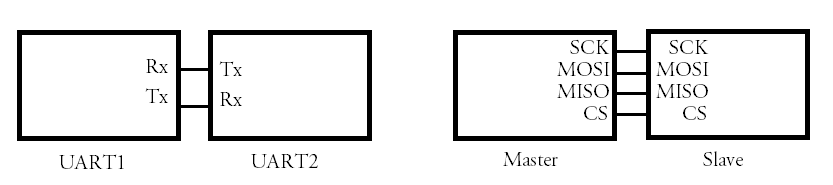
\includegraphics[width=0.8\textwidth]{komunikacija}
  \caption{Serijska i master-slave komunikacija}
  \label{fig:Slika_Komunikacija}
\end{figure}

Kod čitanja stanja push buttona, te kontrole LED dioda, te motora, komunikacija je ostvarena direktnim čitanjem stanja elemenata sistema. Stanje može biti niski napon, odnosno logička nula, ili visoki napon, logička jedinica. Naprimjer, ako je push button pritisnut, on na povezani pin šalje logičku jedinicu, te prema tome sistem započinje kretanje servo motora i očitavanje boje. 

Komunikacija sa mobilnim uređajem ostvarena je uz pomoć bluetooth modula koji je povezan serijski s mikrokontrolerom preko UART modula, kao na lijevoj strani slike \ref{fig:Slika_Komunikacija}. UART modul pretvara paralelni prikazane podatke sa registara u serijski prikazane podatke, odnosno niz bizova. HC-05 modul omogućuje full duplex komunikaciju, odnosno, oba učesnika u komunikaciji mogu biti i prijemnici, i predajnici, te su linije za prijenos i primanje podataka odvojene. Ovaj modul također omogućuje i sinhronu, i asinhronu komunikaciju - i u odgovarajućim, i u nasumičnim intervalima. 

Komunikacija sa modulom za SD karticu ostvarena je preko SPI interfejsa, kao na desnoj strani slike \ref{fig:Slika_Komunikacija}, koji je sinhronog tipa. Kod ovog interfejsa, jedan uređaj je master, odnosno, onaj koji inicira početak prijenosa komunikacije. U ovom slučaju to je mikrokontroler. Modul za SD karticu je slave, te se s njega preko linija za prijenos podataka isti prenose, onda kada master mikrokontroler preko upravljačkih linija to inicira.